\documentclass[thesis.tex]{subfiles}
\begin{document}
\chapter{Future Work}
\label{chap:future-work}

We have described the policies of the mobile ecosystem and how AppPAL can be
used to describe them. We have argued that AppPAL is a good language for
describing these policies, however there are also areas where AppPAL could be
improved to further to describe more kinds of policies and to aid policy
authors, as well as examining further aspects of the mobile ecosystem. This
chapter suggests areas we did not look at and how they might expand our
knowledge of mobile ecosystems and the trust relationships within them.

\section{Plausible SecPAL}

The SecPAL authorization language, and the AppPAL instantiation, allow policy
authors to make use of static analysis tools to make decisions, and allow
principals to make statements about apps through delegation. When these
decisions are made they are made with certainty. If a principal says an app is
safe to access the network then we believe that that principal definitely
believes the app is safe on a network. When a static analysis tool finds that an
app isn't malware then we believe that app to not be malware. This isn't
realistic. Static analysis tools can produce false results. A principal might be
merely fairly confident that an app can access the network safely but not
absolutely certain.

With current authorization languages you cannot quantify the belief a principal
has in any statement. A principal cannot say how \emph{plausible} they think any
statement is.

\subsection{Examples of Plausibility}

SecPAL was designed to make access control decisions. The decision whether to
install allow a user access to a file or not is a binary one: either they can
access it or they cannot. Similarly the decision process for these decisions is
also binary: a user is either logged in or not, a network address is either in
the network or outside it, someone can act as someone else's manager or they can
not. Not all decisions are binary however.

\begin{figure}
  \centering
  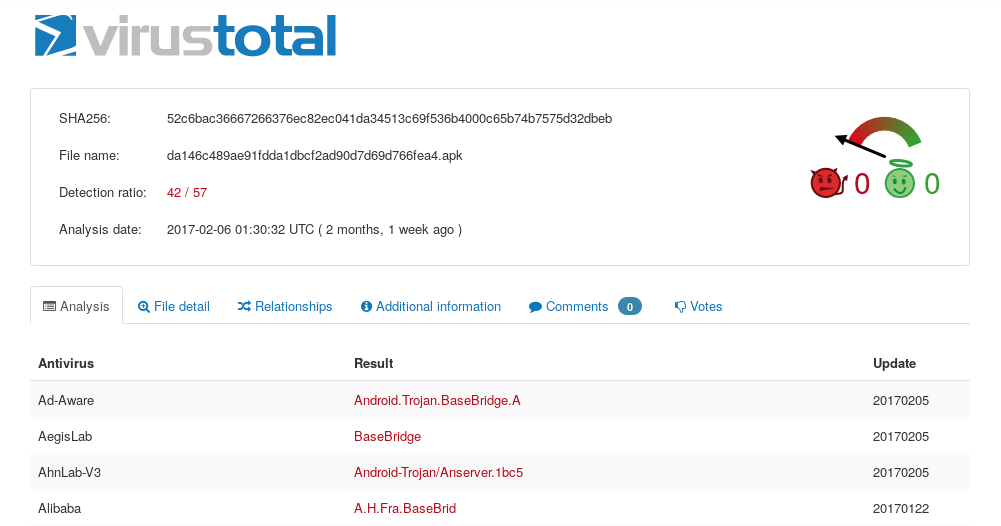
\includegraphics[width=0.49\linewidth]{figures/android-malware.png}
  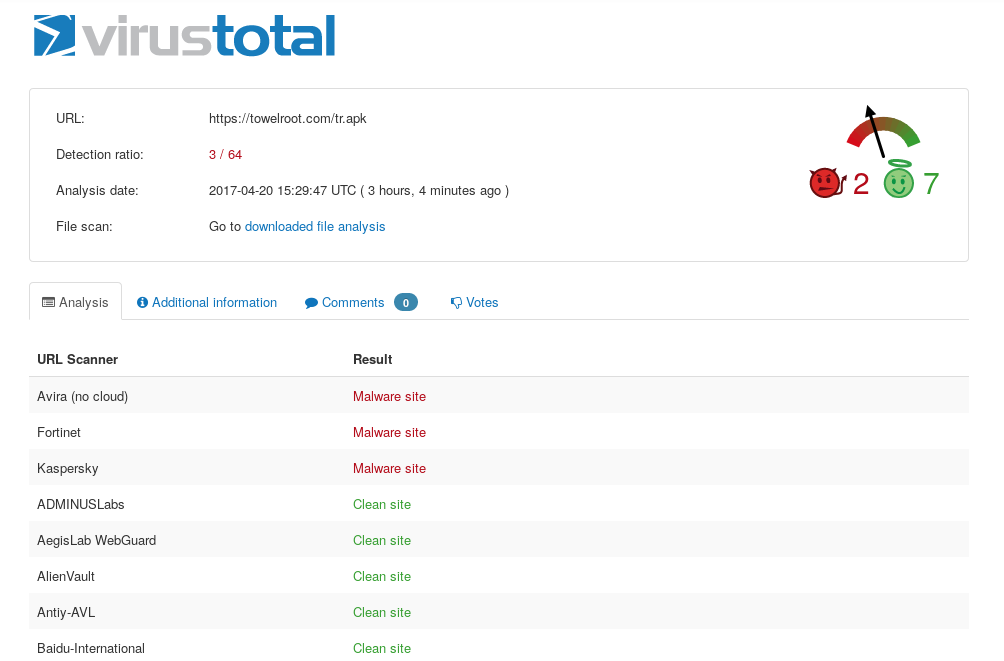
\includegraphics[width=0.49\linewidth]{figures/towelroot.png}
  \caption[VirusTotal results for two Android apps.]{VirusTotal results for 57
    antivirus packages scanning a sample of the BaseBridge Android malware, and 64
    antivirus packages analyzing a download of the (relatively safe) Towelroot
    rooting app.}
  \label{fig:android-malware}
\end{figure}

A user, Alice, may have a policy. That will only install safe apps, ones they
know are not malware. She could use an \ac{AV} program, but these tools are not
infallible. Some change their mind about apps over time. Others are heuristic
based and may only be capable of judging an app based on sufficiently many
malware indicators being present. Instead of using one \ac{AV} program, Alice
opts to use \emph{VirusTotal}; a web service for running files through multiple
\ac{AV} programs. Even for known malware samples VirusTotal rarely gives
absolute answers instead giving the number of \ac{AV} programs that flagged
it~(\autoref{fig:android-malware}). Alice acknowledges this and writes her
policy accordingly:

\begin{lstlisting}
'alice' says App:A isInstallable
  if A isSafe
  with plausibility at least 0.75.

'alice' says 'virustotal' can-say
  App:A isSafe

'virustotal' says 'com.good.app' isSafe
  with plausibility 0.95.

'virustotal' says 'com.malicious.app' isSafe
  with plausibility 0.26.
\end{lstlisting}

She can install the \texttt{com.good.app}, since the plausibility it is good is
greater than her threshold but the \texttt{com.malicious.app} fails her test and
is uninstallable. 

In the first example VirusTotal gave Alice a value for how plausible it was the
app was safe: but what if Alice has to decide this value herself? An example of
this is app recommendations. Alice only wants to install apps that are really
good. She has two friends, Bob and Charlie, who offer her reviews of a game. To
complicate matters further, whilst she trusts Bob utterly, she is a little less
trusting of Charlie.

\begin{lstlisting}
'alice' says App:A isInstallable
  if A isGood
  with plausibility

'bob' says 'com.rovio.angrybirds' isGood
  with plausibility 0.8.

'charlie' says 'com.rovio.angrybirds' isGood
  with plausibility 0.9.

'alice' says 'bob' can-say App:A isGood.

'alice' says 'charlie' can-say App:A isGood
  with plausibility 0.9.
\end{lstlisting}

How should she combine the information to get an overall rating of the game? If
Alice wants to only install an apps that are both good and safe how should she
trade off the plausibility against each other? Is she willing to install a more
dangerous app if it is highly reviewed?

Plausibility is similar to probability (plausibility incorporates the speakers
\emph{belief} that the statement is true as opposed to just its likelihood) and
various papers have proposed probabilistic variants of
Datalog~\cite{fuhr_probabilistic_1995} or explored the semantics of
probabilistic logics~\cite{halpern_analysis_1990}. Role-based access control
languages have incorporated ideas about risk into their
schemes~\cite{josang_analysing_2004,dimmock_using_2004,salim_approach_2011},
which is a similar notion to plausibility and trust. These schemes do not seem
to deal with delegation in the same manner as SecPAL however so incorporating
similar ideas here may be interesting and allow SecPAL and AppPAL greater
expressiveness.

Whilst some work went into developing the ideas behind a plausible SecPAL
variant, we did not finish this work because there are several hard problems
surrounding it. In particular it is far from clear how to combine probabilistic
statements in a consistent, and sound manner. Several choices are possible but
more research is needed to understand the right way to do it and how to develop
Plausible SecPAL into a full, and useful language.


\subsection{Guarantees for Plausible SecPAL} 

In \autoref{appendix:probabilistic} we suggest how we might implement Plausible
SecPAL by modifying Becker~\etal's original design. However we implement it, we
should consider carefully how we might \emph{combine} information and
plausibilities. Combining probabilities of events when you cannot guarantee
independence is hard, and the same is true of plausibility. Strategies such as
taking the product, minimum of combined statements may be too simple. We suggest
the following properties should hold no matter what combination mechanism is
used:

\begin{enumerate}
\item \label{enum:1} If all facts are completely plausible, then evaluation should be
  equivalent to standard SecPAL.
\item \label{enum:0} If any fact is completely  implausible, then it should be equivalent
  to the statement not existing in the assertion context.
\item \label{enum:grow} No derived statement should be more plausible than the conditions used
  to derive it.
\end{enumerate}

Rule~\ref{enum:1} ensures that any plausibility additions do not start to
produce different results to standard SecPAL. We wish to be able to reason about
scenarios where we have partial plausibility, but this addition shouldn't change
our ability to reason when each speaker has total belief in their assertions. If
everything is completely plausible, then the reasoning should be equivalent to
SecPAL where the perfect plausibility is assumed. Similarly if a speaker
believes a fact to be completely implausible then Rule~\ref{enum:0} ensures that
fact is used to derive other facts. SecPAL operates under a \emph{closed world
assumption}, that is that the assertion context contains (or at least can
derive) \emph{all} known facts. If a statement is missing then it is false. If a
speaker believes a statement to be perfectly implausible then it should be
equivalent to falsehood in standard SecPAL and should not be used further.

Rule~\ref{enum:grow} applies to assertions with a conditional part (i.e.~an
\texttt{if}). If this rule were not the case we might be able to grow the
plausibility of a fact by applying a rule that contained its own derived fact in
its condition. For example consider the following rule:
\begin{lstlisting}
'x' says 'y' p
  if 'y' p,
     'z' q.
\end{lstlisting} Say we know already that by applying this rule the plausibility
that \texttt{'x' says 'y' p} will be greater than the plausibility of the
conditionals that \texttt{'x' says 'y' p} and \texttt{'x' says 'z' q}. Since the
decision that \texttt{'x' says 'y' p} is also part of the conditions, we could
repeatedly reapply this rule and raise the plausibility arbitrarily.

\section{Patterns with predicates}

We described in \autoref{chap:apppal} how we split AppPAL predicates into four types: can, has, is and must.
Using the four predicate types we can start to build relationships between them.
We also showed how a policy author could check an obligation was completed when
describing \emph{must} predicates.  Whilst a policy author could write these
rules by hand, AppPAL has tools to automate creating rules like this.

As well as automating creating the policy, we could also start to check other
properties to check the policy is well formed. Using the example of installing
an app; if \emph{Alice says Bob must install
  an app}, then it implies that there should be a rule where \emph{Alice says
Bob has installed that app}.  We might also expect there to be a rule that
\emph{Alice says Bob can install the app}.

This can be taken further: actions where Alice \emph{can} do something might
naturally lead to assertions where Alice \emph{has} done something.  If a policy
author wished to enforce this relationship then we can start to reason about how the
assertion context has changed over time.

\begin{table}\centering
  \begin{tabular}{l c l}
    \toprule
      $F(\phi)$ & $\Rightarrow$ & At sometime in the future $\phi$ is true. \\
      $P(\phi)$ & $\Rightarrow$ & At sometime in the past $\phi$ was true. \\
      $G(\phi)$ & $\Rightarrow$ & $\phi$ will always true. \\
      $H(\phi)$ & $\Rightarrow$ & $\phi$ was always true. \\
    \bottomrule
  \end{tabular}
  \caption{Summary of temporal operators from Prior~\cite{arthur_n._prior_past_1967}.}
  \label{tab:temporal-operators}
\end{table}

Using the temporal operators in \autoref{tab:temporal-operators}, we can start
to write rules expressing the relationship between different predicates. Taking
the earlier example, we might wish to add a rule that if Alice believes Bob has
done something $\phi$, then she must have said he could do that thing in the
past.

\begin{equation*}
  \infer{P\left(\exists AC^\prime~s.t.~AC^\prime, D^\prime \models \mathtt{A~says~B~can~\phi.}\right)}{%
    AC, D \models \mathtt{A~says~B~has~\phi.}}
\end{equation*}

Using this structure we could add a rule to AppPAL that all decisions from the
past, will hold in the future. This might enable us to reduce the size of the
assertion context as once we have a statement that someone \emph{has} we can
remove the respective \emph{can} assertions. Alternatively if we prove the rule
is false, i.e. at no point in the past did Alice permit Bob's action then we can
detect something has gone wrong.

\begin{equation*}
  \infer{\bot}{%
  AC, D \models \mathtt{A~says~B~has~\phi.} & \neg P\left(\exists AC^\prime~s.t.~AC^\prime, D^\prime \models \mathtt{A~says~B~can~\phi.}\right)
  }
\end{equation*}

An AppPAL interpreter might implement this by requiring the \emph{can}
statement be made before any equivalent \emph{has} statement is made. Looking at
a trace from an instance of an AppPAL interpreter with one AC (though which
might import or remove assertions over time), the following trace would be
valid, but if the statement in red was removed it would be rejected.

\begin{center}
  \begin{tabular}{c c l}
    \toprule
    $\vdots$ & $\vdots$ \\
    At $T_i$:   & \textcolor{BrickRed}{$AC_i, D \models \mathtt{A~says~B~can~\phi.}$} & \\
    $\vdots$ & $\vdots$ \\
    At $T_j$:   & $AC_j, D \models \mathtt{A~says~B~has~\phi.}$ & (j $>$ i) \\
    $\vdots$ & $\vdots$ \\
    \bottomrule
  \end{tabular}
\end{center}

Interesting examples are not just limited to \emph{can} and \emph{has}: if Alice
says Bob \emph{must} do some $\phi$, then we would expect that at some point in
the future (if not immediately) that Alice will say that Bob \emph{can} complete
the obligation to $\phi$. Furthermore we would also expect Alice to acknowledge
that at some future point Bob \emph{has} done $\phi$ as she required.

\begin{equation*}
  \infer{F\left(\exists AC^\prime~s.t.~AC^\prime, D^\prime \models \mathtt{A~says~B~has~\phi.}\right)}{%
  F\left(\exists AC^{\prime}~s.t.~AC^{\prime}, D^{\prime} \models \mathtt{A~says~B~can~\phi.}\right) &
    AC, D \models \mathtt{A~says~B~must~\phi.}}
\end{equation*}

Using this interpretation of AppPAL's rules the following for an interpreter
the following trace is valid; but if either statement in red was removed the
interpreter would report an error.

\begin{center}
  \begin{tabular}{c c l}
    \toprule
    $\vdots$ & $\vdots$ \\
    At $T_i$:   & $AC_i, D \models \mathtt{A~says~B~must~\phi.}$ & \\
    $\vdots$ & $\vdots$ \\
    At $T_j$:   & \textcolor{BrickRed}{$AC_i, D \models \mathtt{A~says~B~can~\phi.}$} & \\
    $\vdots$ & $\vdots$ \\
    At $T_k$:   & \textcolor{BrickRed}{$AC_j, D \models \mathtt{A~says~B~has~\phi.}$} & (k $>$ i, k $>$ j) \\
    $\vdots$ & $\vdots$ \\
    \bottomrule
  \end{tabular}
\end{center}

Further investigation into the relationships between predicates, and their
semantics, might allow for interesting auditing possibilities with AppPAL and
extend the language further.

\section{Curation with AppPAL}

We have shown in this dissertation how AppPAL can be used to describe different
policies for BYOD, and for app installation preferences. A logical next step
would be to start to use AppPAL to enforce these policies, and to study how
users might use AppPAL to make decisions.

This could be done by using AppPAL as a mechanism for \emph{curation}. AppPAL
would be used as a tool for finding apps that match user's privacy policies. We
described earlier how we could use AppPAL's \emph{genstore}-framework to build a
curated app store on the basis of a policy. This could be extended to allow for
policy-aware app searches.

\section{AppPAL MDM}

BYOD is another area where it would be interesting to see how AppPAL might be
used in practice. AppPAL is designed to separate the policy specification from
its implementation. By combining an AppPAL policy engine with an MDM package we
could dynamically configure the MDM software to enforce a BYOD policy. This
would allow for greater customization as we could extend the MDM tool to support
contextual and policy driven controls rather than the low-level simple ones that
are the only controls many tools support. More advanced MDM tools, such as
Armando~\etal's \emph{meta-market}~\cite{armando_enabling_2014}, can enforce
more complex policies but cannot distinguish between different contexts. A user
who uses an app for both work and home may wish to run an app unencumbered and
with different accounts when at home compared to at the office. Extending a tool
such as this with AppPAL would allow contextual as well as policy controls into
apps.

Trialing an implementation in a company and working with the IT departments and
policy authors to better understand their needs would allow us to tailor AppPAL
further to implementing BYOD policies rather than just modeling them.

\section{Usability Study}

AppPAL is designed to be readable, but we might guess that most non-technical
users would struggle with writing a formal policy (as they do with many other
technical tasks). Exploring how general users might use policies, either through
a subscription model where they \emph{subscribe} to a policy written by a more
advanced user, or through a graphical interface that helps them build their own
policy, would help us understand how (and in fact whether at all) users would
take advantage of better app controls.

Looking solely at the language a user study with AppPAL should seek to answer at
least three questions looking at a range of users of varying technical skill and
comparing to results from other languages (such as XACML):

\begin{itemize}
\item Can users comprehend the meaning of a policy written in AppPAL? Becker
  designed SecPAL to be readable but didn't trial the language with users.
  Specifically SecPAL was designed to be less verbose than XACML, to abstract away
  the logic-based syntax of the RT family (which some administrators found
  intimidating), and to offer a simple succinct syntax based on natural language.
  Measuring users' comprehension of AppPAL would test whether the syntax offers an
  advantage over other languages.

\item Can users predict the decision made by AppPAL given a policy and a
  scenario? As well as being readable SecPAL was designed to have intuitive
  semantics. We would hope that a user should be able to follow and understand the
  decision process made by AppPAL, but we should test it with users to be sure. A
  key requirement for a policy language should be it's predictability as we do not
  want the language to make surprising decisions (for its users), and allow or
  deny actions that users intuitively believe should not be permitted given a
  policy. Testing whether users can predict decisions given a policy and whether
  they can explain, in high-level terms, the decision process would give some
  measure of the language's intuitiveness.
  
\item Can users modify or create an AppPAL policy given set of requirements? If
  AppPAL is comprehensible and predictable we would hope that a user could tweak
  or even create a policy to meet their own requirements. SecPAL was designed to
  be expressive, but we should test whether users are capable of expressing the
  policies they want using it.
\end{itemize}



\end{document}

%%% local variables:
%%% mode: latex
%%% tex-master: "../ch6.tex"
%%% end:


